% !TeX encoding = UTF-8
%% Простая презентация с примером включения программного кода и
%% пошаговых спецэффектов
\documentclass{beamer}
\usetheme{SPbAU}
%\useoutertheme{infolines}
\usepackage{fontspec}
\usepackage{xunicode}
\usepackage{xltxtra}
\usepackage{xecyr}
\usepackage{hyperref}

%% Minted для подсветки кода
\usepackage[cache=false, outputdir=out]{minted}
\usepackage{listings}

\setminted[kotlin]{xleftmargin=\parindent, linenos, autogobble, frame=lines, escapeinside=\#\#}
\setminted[text]{xleftmargin=\parindent, autogobble, frame=lines, escapeinside=\#\#}

\usepackage{setspace}

\setmainfont[Mapping=tex-text]{DejaVu Serif}
\setsansfont[Mapping=tex-text]{DejaVu Sans}
\setmonofont[Mapping=tex-text]{DejaVu Sans Mono}
\usepackage{polyglossia}
\setdefaultlanguage{russian}
\usepackage{graphicx}
\usepackage{listings}
\lstdefinestyle{mycode}{
  belowcaptionskip=1\baselineskip,
  breaklines=true,
  xleftmargin=\parindent,
  showstringspaces=false,
  basicstyle=\footnotesize\ttfamily,
  keywordstyle=\bfseries,
  commentstyle=\itshape\color{gray!40!black},
  stringstyle=\color{red},
  numbers=left,
  numbersep=5pt,
  numberstyle=\tiny\color{gray},
}
\lstset{escapechar=@,style=mycode}

\newcommand{\code}[1]{\texttt{#1}}

\graphicspath{{img/}}

\definecolor{schema-keyword}{RGB}{0, 0, 128}
\newcommand{\keyword}[1]{\textbf{\textcolor{schema-keyword}{#1}}}

\begin{document}
\title[Cистема эффектов для Kotlin]{Разработка системы условных эффектов с реализацией на языке программирования Kotlin}

\author[Саввинов Д.К.]{Саввинов Дмитрий Кимович\\{\footnotesize\textcolor{gray}{научный руководитель: руководитель команды компилятора языка Kotlin, С.Е. Ерохин}}}
\institute{СПб АУ НОЦНТ РАН}
\frame{\titlepage}

\begin{frame}[fragile]\frametitle{Предметная область. Smartcasts}
\begin{columns}[T]
    \column{0.5\textwidth}
  Работает:

  \begin{minted}{kotlin}
    fun foo(x: Any) {
      if (x is String) {
        println(#\colorbox{green}{x}#.length)
      }
    }
  \end{minted}


  \column{0.5\textwidth}
  Не работает:

  \begin{minted}{kotlin}
  fun isString(x: Any) =
    x is String

  fun foo(x: Any) {
    if (isString(x)) {
     x.#\textcolor{red}{length}#
    }
  }
  \end{minted}
  
  Компилятор не знает, что:
  
  \code{isString(x) == true} $\Leftrightarrow$ \code{x is String}
  
\end{columns}
      
  
  
\end{frame}

\begin{frame}[fragile]\frametitle{Предметная область. Smartcasts}
\begin{columns}[T]
    \column{0.5\textwidth}
    
    Не работает:
    
    \begin{minted}{kotlin}
        fun test(x: Any) {
            assert(x is String)
            x.#\textcolor{red}{length}#
        }
    \end{minted}
    
    \begin{small}
        Компилятор не знает, что:
        
        \code{assert(c)} завершился \\ $\Leftrightarrow$ \\ \code{c == true}
                
    \end{small}
        
    \column{0.5\textwidth}
    
    Не работает:
    
    \begin{minted}{kotlin}
        fun test(list: List<Any>) {
          val ss = list.filter {
              x -> x is String
          }
          ss[0].#\textcolor{red}{length}#
        }
    \end{minted}
    
    \begin{small}
        \setstretch{0.75}
        Компилятор не знает две вещи:
        \begin{itemize}
            \item Лямбда возвращает \code{true} только на \code{String}
            
            \item \code{filter} оставляет только те элементы, на которых лямбда вернула \code{true}
            
        \end{itemize}
    \end{small}
\end{columns}
\end{frame}


\begin{frame}[fragile]\frametitle{Предметная область. Инициализация переменных.}
    \begin{columns}[T]
        \setlength\partopsep{-\topsep}
        \column{0.5\textwidth}
        
        Работает:
        
        \begin{minted}{kotlin}
            val x: Int
            x = 42
            println(x)
        \end{minted}
        
        \column{0.5\textwidth}
        
        Не работает:
        
        \begin{minted}{kotlin}
            val x: Int
            // Reassignment
            run({ #\textcolor{red}{x = 42}# }) 
            
            // Not initialized
            println(#\textcolor{red}{x}#)      
        \end{minted}
        
    \end{columns}
    
    \bigskip
    
      Компилятор знает, что лямбда пишет в \code{x}, но не знает, что она выполнится \textbf{ровно раз}
    
    \bigskip 
    
    Аналогичным образом в Kotlin реализованы \code{synchronized}, \code{try-with-resources}, \code{async-await}, и т.д.
\end{frame}

\begin{frame}\frametitle{Постановка цели и задачи}
    \textbf{Цель:} разработка системы, выполняющей анализ кода на языке программирования Kotlin посредством использования информации о поведении вызываемых функций
    
    \textbf{Требования к системе:} 
    \begin{itemize}
        \item Должна решать как минимум вышеописанные проблемы
        \item Должна быть поддерживаемой
        \item Должна быть расширяемой
    \end{itemize}
    
    \textbf{Задачи:}
    \begin{itemize}
        \item Проанализировать существующие решения
        \item Разработать систему
        \item Реализовать разработанную систему в компиляторе Kotlin
        \item Провести анализ полученного решения, выявить его достоинства и недостатки
    \end{itemize}
\end{frame}

\begin{frame}[fragile]\frametitle{Существующие решения и аналоги}
    \begin{enumerate}
        \item Системы эффектов
        
            \begin{itemize}
                \item \text{<<}An Object-Oriented Effects System>>. Greenhouse, Boyland. 1999
                \item JSR-308 (Checker Framework)
                \item Eff-language
            \end{itemize}
            
        \item Контракты
        
            \begin{itemize}
                \item Контракты в C\#      
                \item Eiffel
                \item Аннотация \code{@Contract} в IDEA
            \end{itemize}
        
        \item Языки спецификации
            
            \begin{itemize}
                \item The Z Notation                
                \item ANSI C Specification Language                
                \item Larch
            \end{itemize}
    \end{enumerate}
\end{frame}

\begin{frame}\frametitle{Решение. Основные понятия}
    \begin{definition}
        \textbf{Эффект вычисления} -- некоторая информация о состоянии окружения, полученная в результате исполнения данного вычисления
    \end{definition}
    
    \begin{itemize}
        \item Запись в переменную -- эффект
        \item И возвращение значения -- тоже эффект!
        \item И даже если мы просто узнали тип какой-то переменной, это тоже эффект!
    \end{itemize}
\end{frame}

\begin{frame}\frametitle{Решение. Основные понятия}
    \begin{definition}
        \textbf{Схема эффектов} -- описание эффектов вычислений и \emph{условий}, вызывающих эти эффекты.
    \end{definition}
    
    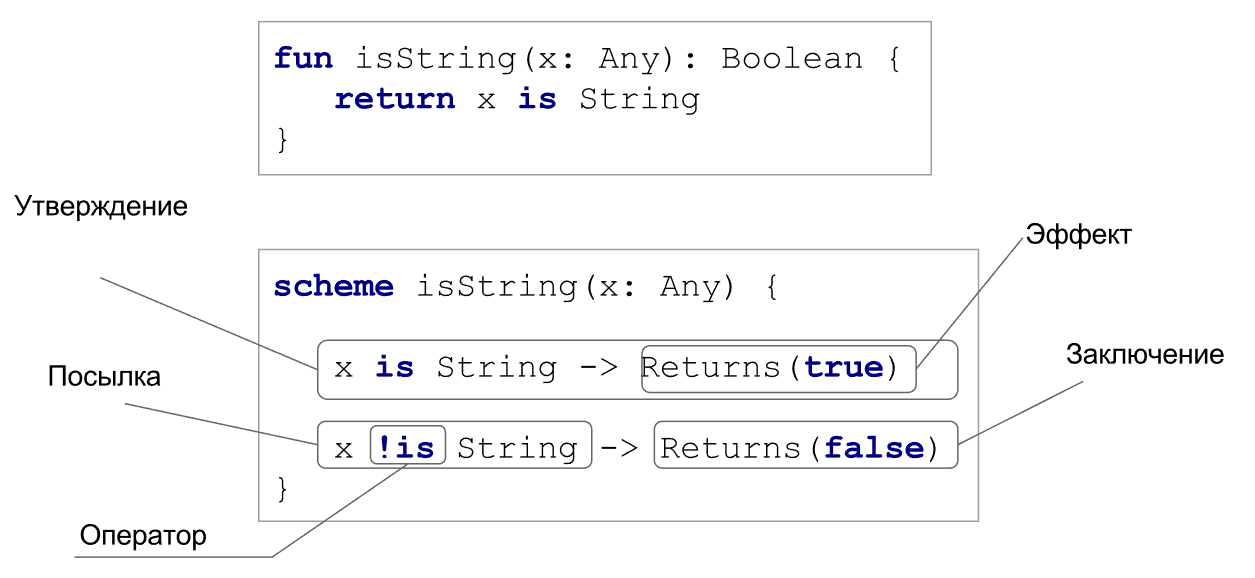
\includegraphics[scale=0.25]{schema-anatomy}
\end{frame}
    
\begin{frame}[fragile, t]\frametitle{Комбинирование схем. Постановка проблемы}
    \setlength\partopsep{-\topsep}
    
    Даны две схемы:
    
    \vskip0.0em
    \begin{columns}[T]
        \column{0.5\textwidth}
        \begin{minted}[fontsize=\scriptsize]{text}
            #\keyword{schema}# isString(x: Any) {
               x #\keyword{is}# String  -> Returns #\keyword{true}#
               x #\keyword{!is}# String -> Returns #\keyword{false}#
            }
            
        \end{minted}
        
        \column{0.5\textwidth}        
        \begin{minted}[fontsize=\scriptsize]{text}
            #\keyword{schema}# assert(c: Bool) {
              с == #\keyword{true}# -> Returns #\keyword{true}#
              с != #\keyword{true}# -> 
                   Throws AssertionError
            }         
        \end{minted}
    \end{columns}
   
    Пусть выполняется \textbf{вложенный} вызов: \code{assert(isString(x))}
    
    \bigskip
    Хотелось бы получить \textbf{комбинированную} схему для этого вызова:
    
    \begin{minted}[fontsize=\small]{text}
        #\keyword{scheme}# assert(isString(x)) {
          x #\keyword{is}# String  -> Returns #\keyword{true}#
          x #\keyword{!is}# String -> Throws AssertionError
        }        
    \end{minted}
\end{frame}

\begin{frame}[fragile]\frametitle{Комбинирование схем. Общее решение}
    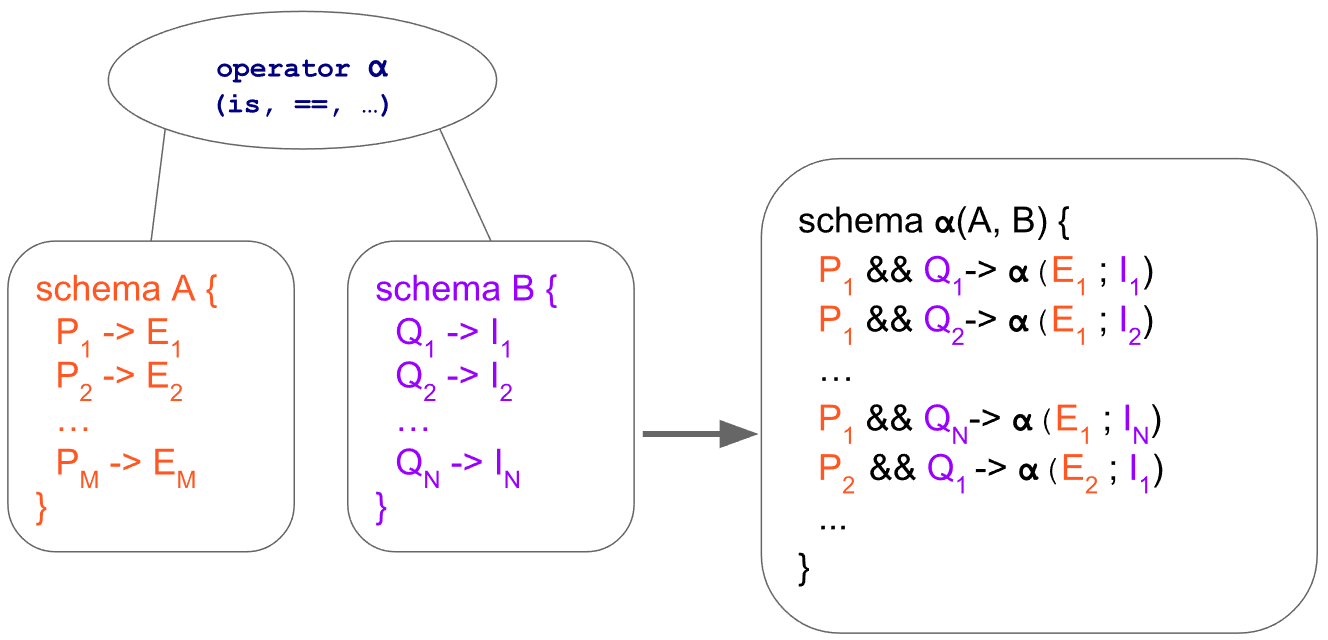
\includegraphics[scale=0.25]{schema-flatten}
    
    \begin{itemize}
        \item Преобразование $\alpha$ определяется оператором
        \item Как правило, определяется достаточно тривиально и \emph{только на небольшом классе} эффектов
        \begin{itemize}
            \item \code{==(Returns x; Returns y)} $\equiv$ \code{Returns(x == y)}
        \end{itemize}
    \end{itemize}
\end{frame}

\begin{frame}[fragile]\frametitle{Комбинирование схем. Частичные вычисления}
    \setbeamertemplate{caption}{\raggedright\insertcaption\par}
    \small
    \begin{figure}
        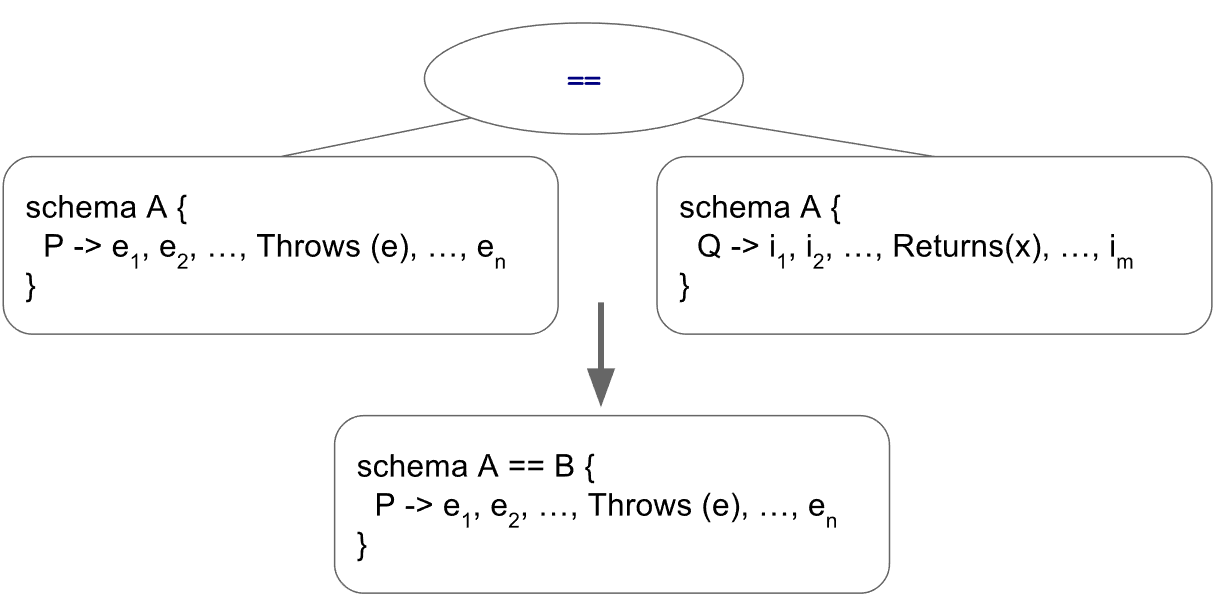
\includegraphics[scale=0.20]{schema-outcomes-flatten}
        \caption{Эффекты правой части не успели выполниться!} 
    \end{figure}
    
    \vskip-1.0em
    \begin{definition}
        \textbf{Исход} -- специальный класс эффектов (\code{Returns} и \code{Throws}), которые говорят об успешности вычислений. Система эффектов <<знает>> про все исходы.
     
    \end{definition}   
\end{frame}

\begin{frame}[fragile, t]\frametitle{Реализация. Источники схем эффектов}
        \setlength\partopsep{-\topsep}
    \begin{itemize}
        \item Явная аннотация на функции
        
        \begin{minted}{kotlin}
            @Effects("""
              condition == true -> Returns unit;
              condition != true -> Throws AssertionError
            """)
            fun myAssert(condition: Boolean): Unit {
              if (!condition) 
                throw AssertionError("Assertion failed")
            }    
        \end{minted}
        
        \item Вывод из тела функции
        
        В текущей реализации поддерживаются только тела, состоящие из одного выражения (expression):
        
        \begin{minted}{kotlin}
            fun isString(x: Any?) = x is String
        \end{minted}
    \end{itemize}
\end{frame}

\begin{frame}[fragile, t]\frametitle{Реализация. Полный алгоритм}
    Пусть дан вызов \code{foo(1, bar(s, null))}. 
    
    \begin{enumerate}
        \item Из IR компилятора убирается лишняя информация, проверяется, что resolving выполнен, и т.д.
        \item Все вызовы заменяются на соответствующие схемы, выполняется подстановка переменных
    \end{enumerate}
    
    \begin{figure}
            \centerline{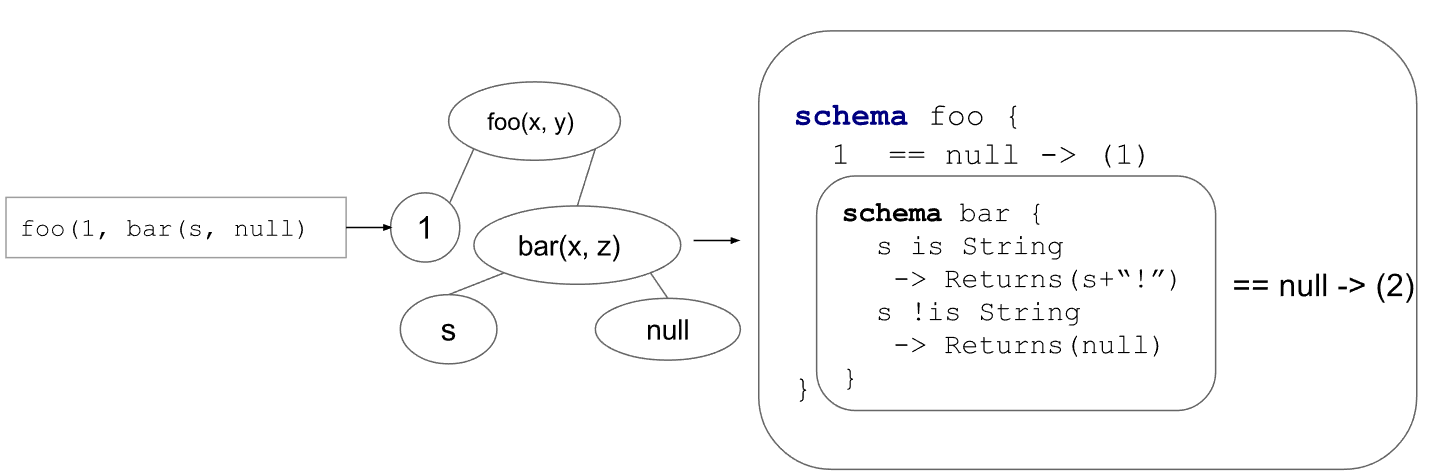
\includegraphics[width=\paperwidth]{pipeline-1}}
    \end{figure}
\end{frame}

\begin{frame}[t]\frametitle{Реализация. Полный алгоритм}
    
    \begin{enumerate}
    \setcounter{enumi}{3}

      \item Выполняется комбинирование схем, получаем одну большую схему, описывающую все эффекты данного вызова
      \item Выполняется сокращение схемы: вычисляются константы, откидываются невозможные ветки вычислений и т.д.
    \end{enumerate}
    
    \centerline{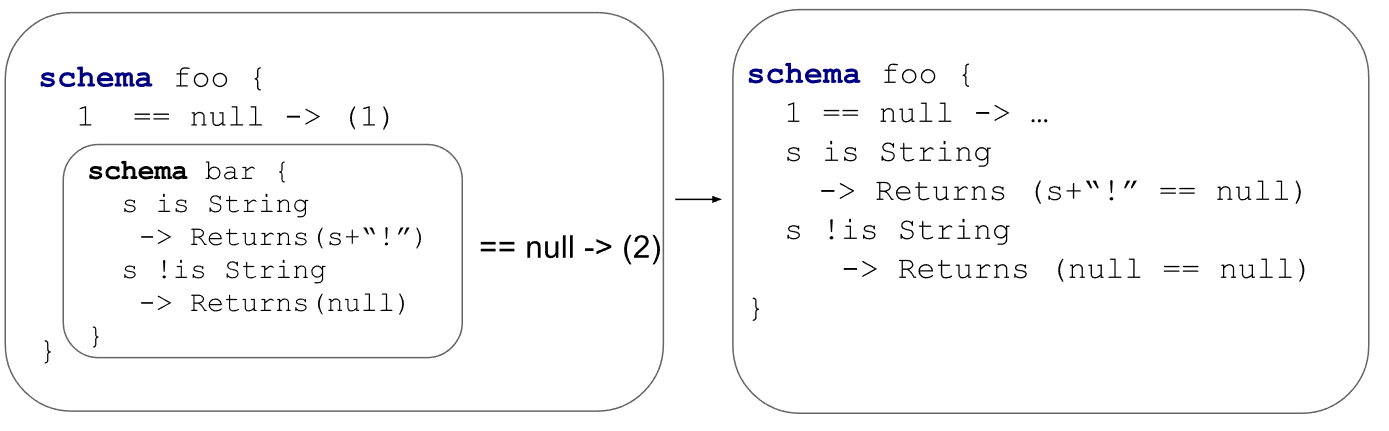
\includegraphics[width=\paperwidth]{pipeline-2} }
\end{frame}

\begin{frame}[fragile, t]\frametitle{Применение. Детерминированные вызовы}
    Вводим эффект \code{Calls(f, c)}: <<Функция $f$ будет вызвана $c$ раз>>
    
    \begin{columns}[T]
        \column{0.5\textwidth}
        
        \begin{minted}[fontsize=\small]{kotlin}
            fun run(block: () -> Unit) 
                = block()          
        \end{minted}
        
                
        \column{0.5\textwidth}
        
        \begin{minted}{text}
            #\keyword{schema}# run {
              #\keyword{true}# -> Calls(block, 1)
            }
        \end{minted}
    \end{columns}
    
    \bigskip
    Данный эффект <<хороший>> в том смысле, что он -- классический \emph{side-effect}.
    
    Поэтому он легко описывается и не требует дополнительных конструкций при введении
\end{frame}

\begin{frame}[fragile, t]\frametitle{Применение. Смарткасты в коллекциях}
    Для введения смарткастов в коллекциях нам понадобится два дополнительных оператора:
    
    \begin{itemize}
        \item \code{S at Y}, где $S$ -- схема, $Y$ -- эффект
        
        \centerline{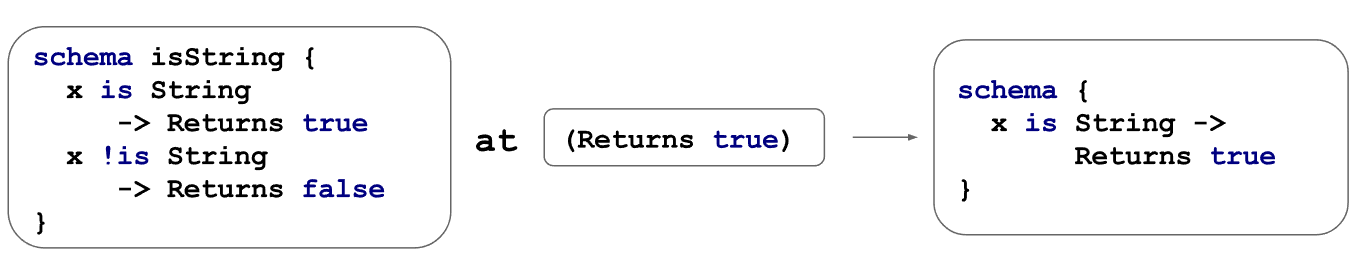
\includegraphics[width=\paperwidth]{at-operator}}
        
        \item \code{S typeOf V}, где $S$ -- схема, $V$ -- переменная
        
        \centerline{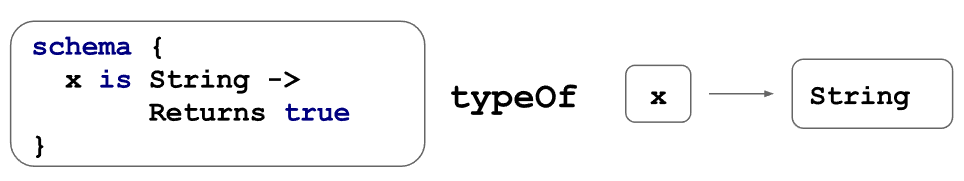
\includegraphics[width=\paperwidth]{typeof-operator}}
    \end{itemize}
\end{frame}

\begin{frame}[fragile, t]\frametitle{Применение. Смарткасты в коллекциях}
    \begin{minted}[fontsize=\small]{kotlin}
        fun filter(l: List<T>, p: (x: T) -> Boolean): List<T> {
            ...
        }
    \end{minted}
    
    \begin{minted}{text}
        #\textbf{\textcolor{schema-keyword}{schema}}# filter {
          true -> Returns List < 
                    #$\big($# #\textit{p(x)}# #\keyword{at}# (Returns #\keyword{true}#) #$\big)$# #\keyword{typeOf}# x 
                    #\footnotesize{тип переменной x, если p(x) вернул true}#
               >
        }
    \end{minted}
\end{frame}

\begin{frame}[fragile, t]\frametitle{Итоги}
    \begin{itemize}
        \item Была разработана грамматика, написан парсер с помощью ANTLR
        \item Были разработаны правила комбинирования схем эффектов
        \item Были поддержаны некоторые виды эффектов: \code{Returns}, \code{Throws}, \code{Calls}
        \item Были улучшен статический анализ языка Kotlin:
            \begin{itemize}
                \item Смарткасты в условных выражениях, assert-подобных вызовах, коллекциях
                \item Анализ (ре)инициализации переменных
            \end{itemize}
       \item Система расширяема за счет добавления новых эффектов и операторов
       \item Поддерживается вывод эффектов для отдельных выражений (expressions)
    \end{itemize}
\end{frame}

\begin{frame}\frametitle{Дальнейшие планы}
    \begin{itemize}
        \item Внесение системы master-ветку компилятора Kotlin
        \item Аннотация стандартной библиотеки Kotlin
        \item Вывод эффектов по телу функции
        \item Исследование полезности более мощных понятий мат. логики (например, кванторы)
        \item Исследование полезности других эффектов (ввод-вывод, многопоточность)
    \end{itemize}
\end{frame}
\end{document}

